\documentclass{beamer}
\usepackage[utf8]{inputenc} 
\title{Paweł Śpiewak}
\author{Patryk Kowalewski}
\institute{UWM}
\date{\today}
\usepackage{amsfonts}
\usepackage[MeX]{polski}
\begin{document}
\frame{\titlepage}

\begin{frame}
\frametitle{Spis Treści}
\tableofcontents
\end{frame}

\section{Życiorys}
\begin{frame}{Życiorys Pawła Śpiewaka}
\begin {itemize}
\item Paweł Śpiewak (ur.17 kwietnia 1951) --- polski socjolog, doktor habilitowany nauk humanistycznych, profesor nadzwyczajny Uniwersytetu Warszawskiego.
\end {itemize}
\end{frame}

\begin{frame}{Zdjęcie}

\begin{figure}[here]
\begin{center}
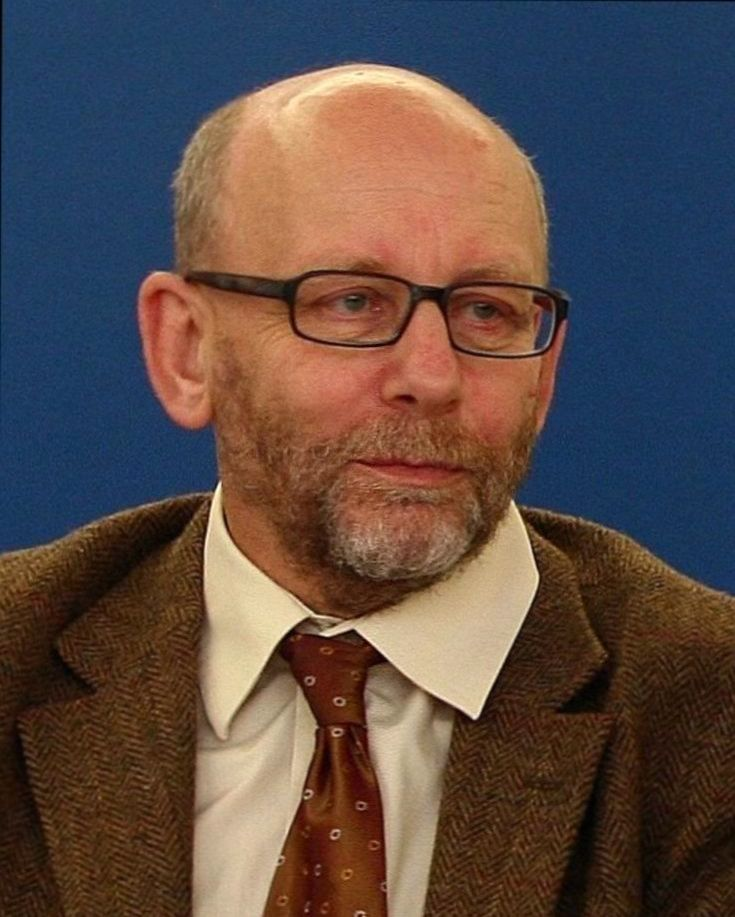
\includegraphics[scale=0.6]{pawcio.jpg}
\end{center}
\end{figure}

\end{frame}

\begin{frame}{Życiorys cd.}
\begin {itemize}
\item<1> W~1984 uzyskał stopień doktora. W~2000 został doktorem habilitowanym.
\pause
\item<2>3~października 2011 otrzymał nominację na stanowisko dyrektora Żydowskiego Instytutu Historycznego.
\item<3> W~2013 otrzymał Nagrodę im. księdza Józefa Tischnera w kategorii „pisarstwo religijne lub filozoficzne” za całokształt twórczości.
\end {itemize}
\end {frame}

\section{Twórczość}
\begin{frame}{Twórczość naukowa i publicystyczna}
Zajmuje się socjologią ogólną, socjologią polityki, historią myśli i filozofii społecznej oraz politycznej. Jest autorem prac naukowych z tych dziedzin.
\end {frame}

\begin{frame}{Twórczość naukowa i publicystyczna cd.}
Jest członkiem Stowarzyszenia Pisarzy Polskich. Był w~kolegiach redakcyjnych. Publikował także w~wielu gazetach codziennych.Jest też stałym współpracownikiem „Tygodnika Powszechnego”.
\end {frame}

\begin{frame}{Twórczość naukowa i publicystyczna cd.}
Ponadto efektem jego zainteresowania Biblią jest publikacja książkowa Midrasze: Księga nad Księgami, za którą został nominowany do Nagrody Literackiej Nike~2005.
\end {frame}

\section{Publikacje}
\begin{frame}{Wybrane publikacje:}
\begin {itemize}
\pause
\item Gramsci, 1977 \pause
\item Ideologie i obywatele, 1991 \pause
\item W stronę wspólnego dobra, 1998 \pause
\item Anti-Totalitarismus. Eine polnische Debatte, 2003 \pause
\item Obietnice demokracji, 2004 \pause
\item Midrasze: księga nad księgami, 2004 \pause
\item Pamięć po komunizmie, 2005 \pause
\item Pięć ksiąg Tory, 2012 \pause
\item Żydokomuna, 2012 
\end {itemize} 
\end {frame}

\section{Koniec}
\begin{frame}{Koniec informacji}
\begin {itemize}
\item Koniec
\end {itemize}
\end {frame}

\section{Bibliografia}
\begin{frame}{Bibliografia}
Bibliografia:
\begin{thebibliography}{9}
\bibitem{deni}
--Wikipedia, Paweł Śpiewak
\end{thebibliography}
\end{frame}

\end{document}